\documentclass[aspectratio=169,12pt]{beamer}
\usepackage[utf8]{inputenc}
\usepackage[english]{babel}
\usepackage{wrapfig}
%\usepackage{siunitx}

\usepackage{multicol}
\usepackage{mathtools}

\usepackage[normalem]{ulem}

\pagestyle{empty}

\usepackage{pgf,tikz}
\usepackage{pgfplots}
\usetikzlibrary{matrix}
\usetikzlibrary{arrows}

%\usepackage{wrapfig}
\mode<presentation>
\usefonttheme{professionalfonts}
\usetheme{Darmstadt}
\usecolortheme{orchid}
\useoutertheme{default}
\setbeamertemplate{headline}{}

\renewcommand{\baselinestretch}{1.1}

%gets rid of bottom navigation bars
\setbeamertemplate{footline}[page number]

%gets rid of navigation symbols
\setbeamertemplate{navigation symbols}{}

%\frameframe{none} % No default frame

%\setlength{\framewidth}{8.7in} \setlength{\frameheight}{7.2in}

\parindent 0pt
\setlength{\parskip} {1ex plus 0.5ex minus 0.2ex}


%\usepackage[bbgreekl]{mathbbol}
\usepackage{amsfonts}

%\DeclareSymbolFontAlphabet{\mathbb}{AMSb}
%\DeclareSymbolFontAlphabet{\mathbbl}{bbold}

\newcommand{\Sym}{{\mathcal S}}
\DeclareMathOperator{\Aut}{Aut}
\DeclareMathOperator{\Tr}{Tr}
\DeclareMathOperator{\trace}{Trace}
\DeclareMathOperator{\range}{range}
\DeclareMathOperator{\rank}{rank}

\usepackage{breqn}
\usepackage{multicol}
\usepackage{colortbl}
\usepackage{lmodern}
\usepackage{tabularx}
\usepackage{multirow}
\usepackage{amssymb}
\usepackage{amsmath}
\usepackage{stmaryrd}
\usepackage{color}
\usepackage{graphicx}
\graphicspath{ {img/} }
\usepackage{hyperref}

\input{epsf}
\title{Introducción}
\author{}

\DeclareMathOperator{\Hom}{Hom}
\DeclareMathOperator{\sing}{sing}

\DeclareMathOperator{\chara}{char}
\DeclareMathOperator{\Jacob}{Jacob}
\DeclareMathOperator{\Sing}{Sing}
\newcommand{\fracNoLine}[2]{\genfrac{}{}{}{0pt}{#1}{#2}}

%\beamerdefaultoverlayspecification{<+->}

\usepackage{listings,xcolor,bm}


\definecolor{mygreen}{rgb}{0,0.6,0}
\definecolor{mygray}{rgb}{0.5,0.5,0.5}
\definecolor{mymauve}{rgb}{0.58,0,0.82}
\lstset{
  backgroundcolor=\color{white},   % choose the background color; you must add
  basicstyle=\small\ttfamily,      % the size of the fonts that are used for the code
  breakatwhitespace=false,         % sets if automatic breaks should only happen at whitespace
  breaklines=true,                 % sets automatic line breaking
  captionpos=b,                    % sets the caption-position to bottom
  commentstyle=\color{mygreen},    % comment style
  deletekeywords={...},            % if you want to delete keywords from the given language
  escapeinside={\%*}{*)},          % if you want to add LaTeX within your code
  extendedchars=true,              % lets you use non-ASCII characters; for 8-bits encodings only, does not work with UTF-8
  firstnumber=1,                % start line enumeration with line 1000
  frame=single,	                   % adds a frame around the code
  keepspaces=true,                 % keeps spaces in text, useful for keeping indentation of code (possibly needs columns=flexible)
  keywordstyle=\color{blue},       % keyword style
  language=Python,                 % the language of the code
  morekeywords={*,...},            % if you want to add more keywords to the set
  numbers=left,                    % where to put the line-numbers; possible values are (none, left, right)
  numbersep=5pt,                   % how far the line-numbers are from the code
  numberstyle=\tiny\color{mygray}, % the style that is used for the line-numbers
  rulecolor=\color{black},         % if not set, the frame-color may be changed on line-breaks within not-black text (e.g. comments (green here))
  showspaces=false,                % show spaces everywhere adding particular underscores; it overrides 'showstringspaces'
  showstringspaces=false,          % underline spaces within strings only
  showtabs=false,                  % show tabs within strings adding particular underscores
  stepnumber=5,                    % the step between two line-numbers. If it's 1, each line will be numbered
  stringstyle=\color{mymauve},     % string literal style
  tabsize=4,	                   % sets default tabsize to 2 spaces
  title=\lstname                   % show the filename of files included with \lstinputlisting; also try caption instead of title
}

\begin{document}

\newtheorem{prop}{Proposici\'on}
\newtheorem{algo}[prop]{Algorithm}
\newtheorem{teor}[prop]{Theorem}
\newtheorem{lema}[prop]{Lemma}
\newtheorem{coro}[prop]{Corollary}
\newtheorem{defi}[prop]{Definition}

\newcommand{\ideal}[1]{{\left\langle{#1}\right\rangle}}
\newcommand{\demo}{\textbf {Demostraci\'on. }}
\newcommand{\obse}{\textbf {Observaci\'on. }}
\newcommand{\Input}{\textbf {Input: }}
\newcommand{\Output}{\textbf {Output: }}
\newcommand{\Examp}{\textbf {Ejemplo }}
\newcommand{\Examps}{\textbf {Ejemplos }}

\newcommand{\kk}{{\mathbbl k}}
\newcommand{\V}{{\mathbf V}}
\newcommand{\I}{{\mathbf I}}
\newcommand{\PP}{{\tilde P}}
\newcommand{\QQ}{{\tilde Q}}

\newcommand{\F}{{\mathbb F}}
\newcommand{\Q}{{\mathbb Q}}
\newcommand{\N}{{\mathbb N}}
\newcommand{\R}{{\mathbb R}}
\newcommand{\Z}{{\mathbb Z}}
\newcommand{\CC}{{\mathbb C}}
\newcommand{\eLL}{{\mathcal L}}



\newcommand{\MinAss}{\textrm {MinAss}}
\newcommand{\Ass}{\textrm {Ass}}
\newcommand{\mcm}{\textrm {mcm}}
\newcommand{\mcd}{\textrm {mcd}}
%\newcommand{\mod}{\textrm { mod }}
\newcommand{\lt}{\textrm {lt}}
\newcommand{\Lt}{\textrm {Lt}}
\newcommand{\lp}{\textrm {lp}}
\newcommand{\lc}{\textrm {lc}}
\newcommand{\lm}{\textrm {lm}}
\newcommand{\barra}{\ /\ }
\newcommand{\multideg}{\textrm {multideg}}

\newcommand{\sep}{\textrm {sep}}
\newcommand{\Syz}{\textrm {Syz}}
\newcommand{\n}{\~n}
\newcommand{\cG}{\textrm {cG}}
\newcommand{\dG}{\textrm {dG}}
\newcommand{\nG}{\textrm {nG}}
\newcommand{\CE}{\textrm {CE}}
\newcommand{\CG}{\textrm {CG}}
\newcommand{\CF}{\textrm {CF}}
\newcommand{\DG}{\textrm {DG}}
\renewcommand{\NG}{\textrm {NG}}

\newcommand{\p}{{\boldsymbol{p}}}
\newcommand{\q}{{\boldsymbol{q}}}

\newcommand{\X}{{\boldsymbol{X}}}
\newcommand{\x}{{\boldsymbol{x}}}
\renewcommand{\u}{{\boldsymbol{u}}}
\renewcommand{\t}{{\boldsymbol{t}}}
\renewcommand{\a}{{\boldsymbol{a}}}
\renewcommand{\b}{{\boldsymbol{b}}}
\renewcommand{\c}{{\boldsymbol{c}}}

%Titulos en espa�ol
%\renewcommand{\chaptername}{Cap\'{\i}tulo}
%\renewcommand{\bibname}{Bibliograf\'{\i}a}

\newcommand{\kring}{\kk[\x]}
\newcommand{\kRing}{\kk[X]}
\newcommand{\qring}{\Q[\x]}

%\renewcommand\itemindent{-10pt}
%\renewcommand{\theenumi}{\arabic{enumi}}
%\renewcommand{\labelenumi}{\Alph{enumi}}

\definecolor{issac}{rgb}{1.00,0.00,0.00}
%------------------------------------------------------------------

\begin{frame}

 \begin{center}

\Large\textbf{Laboratorio de Datos} \\
\large\textbf{Visualización}
%\vspace{0.5cm}

% \textit{Santiago Laplagne} \\
%slaplagn@dm.uba.ar \\


%\vspace{0.5cm}
%{\small Trabajo en progreso en conjunto con \emph{Jose Capco} (Universit\"at Innsbruck) y \emph{Claus Scheiderer} %(Universit\"at Konstanz).} \\

\vspace{1cm}
Primer Cuatrimestre 2024 \\ Turnos tarde y noche

\vspace{1cm}


 {\small Facultad de Ciencias Exactas y Naturales, UBA}
 \end{center}


\end{frame}

%------------------------------------------------------------------

\begin{frame}
\frametitle{Gramática de Gráficos}

\begin{minipage}{.55\textwidth}
La Gramática de Gráficos es un marco para pensar sobre la visualización desarrollado por Leland Wilkinson. Su idea central es que cualquier visualización se puede descomponer en varias partes constituyentes.

\vspace{0.5cm}

Referencia:
\begin{itemize}
\item "The Grammar of Graphics (Statistics and Computing)", Leland Wilkinson. 
\end{itemize}
\end{minipage} %
\begin{minipage}{.4\textwidth}
\begin{center}
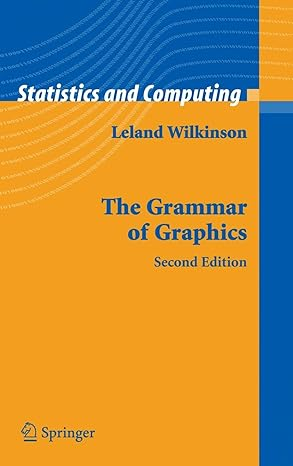
\includegraphics[scale=0.35]{TheGrammarOfGraphics.jpg}
\end{center}
\end{minipage}

\end{frame}

%------------------------------------------------------------------

\begin{frame}
\frametitle{Elementos de un gráfico}

\textbf{1) Los datos}

En el centro de cualquier visualización, por supuesto, están los datos que se esperaban visualizar.

\textbf{2) Las marcas}

Para visualizar nuestros datos, debemos representar los datos con marcas reales en nuestra figura. 

Estos incluyen no sólo los ejes que dan forma a nuestra figura, sino también puntos, círculos, barras u otras formas geométricas.

\end{frame}

%------------------------------------------------------------------

\begin{frame}
\frametitle{Elementos de un gráfico}

\textbf{3) La codificación (o mapeo o mapping)}

Para vincular nuestros datos a las marcas en nuestra figura, debemos decidir sobre un mapeo de datos a marcas. Esta codificación de datos en características visuales es donde ocurre la magia.

\textbf{4) Canales}

Las características visuales de nuestro gráfico en las que podemos codificar información se denominan "canales". 

Algunos canales son obvios: un canal puede ser la ubicación de puntos a lo largo del eje x, otro canal es la ubicación de puntos a lo largo del eje y.

Hay otros canales en los que también podemos codificar datos, como el tamaño, la forma o el color de los puntos.

\end{frame}

%------------------------------------------------------------------

\begin{frame}
\frametitle{Gramática de Gráficos - Ejemplo}

\begin{center}
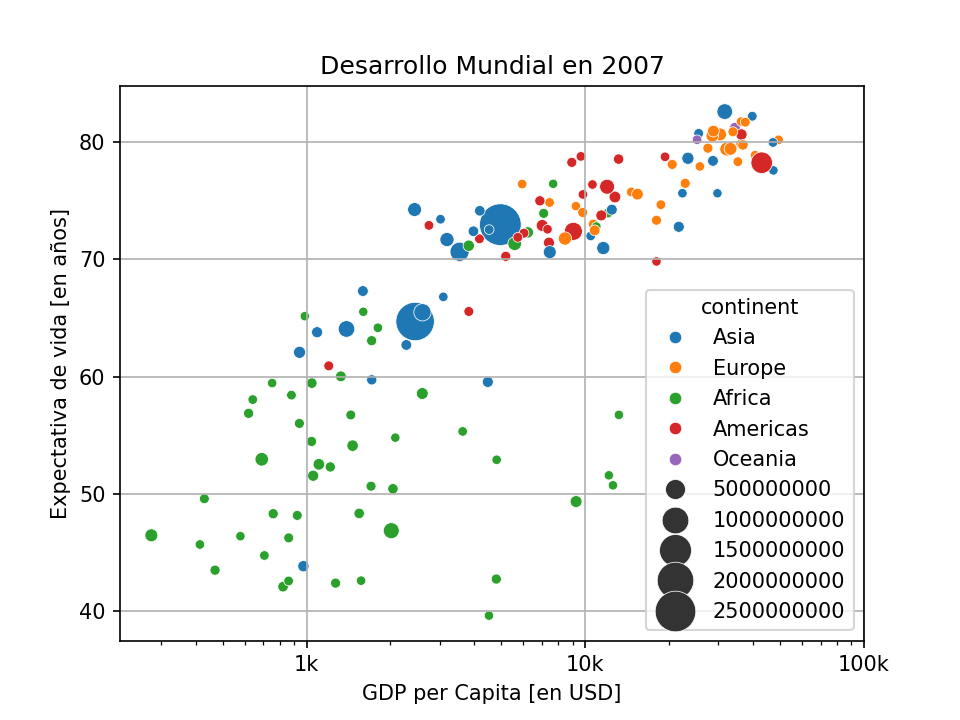
\includegraphics[scale=0.5]{desarrollo2007.png}
\end{center}

Canales: coordenada en el eje $X$, coordenada en el eje $Y$, tamaño y color.
\end{frame}

%------------------------------------------------------------------

\begin{frame}
\frametitle{Seaborn objects en Python}

\begin{minipage}{.55\textwidth}
Introducido a finales de 2022, el nuevo sistema está basado en el paradigma "Gramática de Gráficos" que utilizan otros paquetes como \lstinline{ggplot2} de R.

No necesitamos recordar una docena de métodos para hacer gráficos, todo gráfico se hace mediante una única clase \lstinline{Plot()}.

\vspace{0.5cm}

Seaborn es una biblioteca de visualización construida sobre \lstinline{matplotlib}, para interactuar en forma más amigable.

\end{minipage} \hspace{1cm} %
\begin{minipage}{.35\textwidth}
\begin{center}
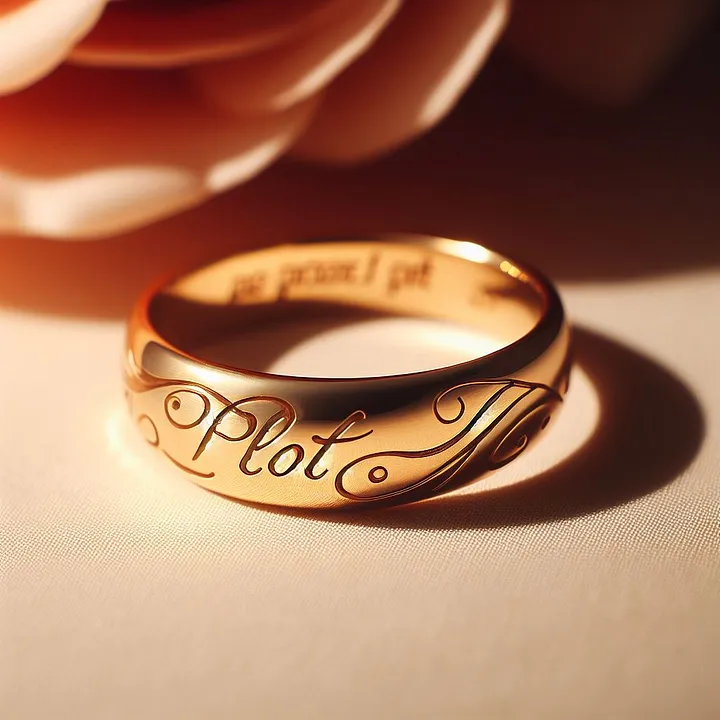
\includegraphics[scale=0.20]{PlotRing.png}
\end{center}
\end{minipage}


\end{frame}

%------------------------------------------------------------------

\begin{frame}
\frametitle{Mapeo y asignación por capas}

\begin{itemize}
\item Si asignamos una codificación (o mapeo) al definir un Plot(),
el mapeo se asigna en todas las capas de marcas (objetos mark). 
\item Si asignamos una codificación dentro del método add() de una marca, el mapeo se realiza solo en esa capa. 
\item Si asignamos un parámetro de la marca, el valor se asigna directamente (no es una codificación de datos).
\end{itemize}

\begin{center}
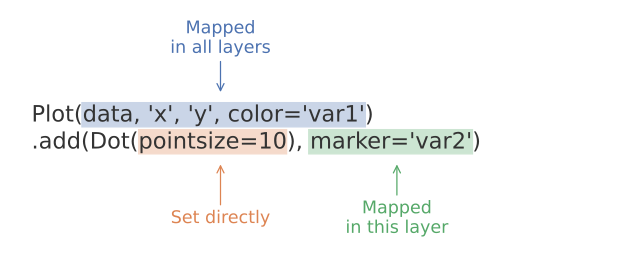
\includegraphics[scale=0.40]{practica3-img-mappings.png}
\end{center}

\end{frame}


%------------------------------------------------------------------

\begin{frame}
\frametitle{Distintos gráficos}

Vimos hasta ahora:

\begin{itemize}
\item \textbf{Curvas.} Se utilizan para representar funciones, para cada valor de la variable en el eje $x$ tengo un único valor de la variable en el eje $y$.
\item \textbf{Gráficos de dispersión (scatter plot).} Se grafican puntos en el plano, para analizar la relación entre dos variables numéricas. Para cada valor de $x$ puede haber varios valores de $y$.
\end{itemize}

\end{frame}


%------------------------------------------------------------------

\begin{frame}
\frametitle{Gráfico de barras}

\begin{minipage}{.55\textwidth}
Un \textbf{gráfico de barras} muestra la relación entre una variable categórica y una variable numérica. A cada valor de la variable categórica corresponde una barra. El tamaño de la barra representa el valor númerico correspondiente al dato categórico.
\end{minipage} \hspace{1cm} %
\begin{minipage}{.35\textwidth}
\begin{center}
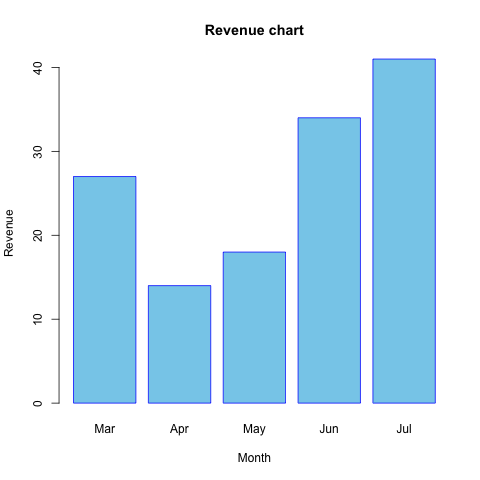
\includegraphics[scale=0.30]{clase4-barchart_months_revenue_sample.png}
\end{center}
\end{minipage}
\end{frame}


%------------------------------------------------------------------

\begin{frame}
\frametitle{Histograma}

\begin{minipage}{.55\textwidth}
Un \textbf{histograma} puede pensarse como un caso particular de gráfico de barras, para una serie de datos de una variable numérica o categórica.

En el eje $x$ representamos los valores de una variable categórica o intervalos (del mismo tamaño) de una variable numérica.

El tamaño de la barra representa la cantidad de veces que se repite cada valor de la variable categórica en la serie, o la cantidad de veces que el valor de la serie cae en cada uno de los intervalos.
\end{minipage} \hspace{1cm} %
\begin{minipage}{.35\textwidth}
\begin{center}
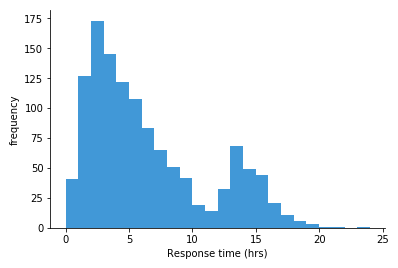
\includegraphics[scale=1.5]{clase4-histogram-example-1.png}
\end{center}
\end{minipage}
\end{frame}


%------------------------------------------------------------------

\begin{frame}
\frametitle{Box plot}

Un gráfico \textbf{box plot} usa cajas y líneas para mostrar información de la distribución de uno o más grupos de datos numéricos.

\begin{center}
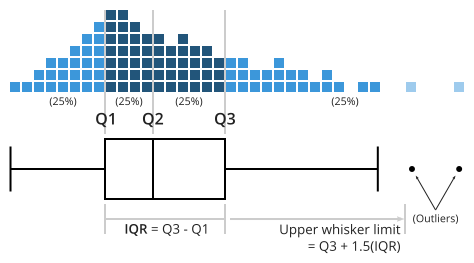
\includegraphics[scale=.5]{clase4-box-plot-construction.png}
\end{center}

\end{frame}

%------------------------------------------------------------------

\begin{frame}
\frametitle{Elementos de un Box plot}

Dada una variable numérica, ordenamos los valores y los partimos en 4 grupos de igual tamaño.

\begin{itemize}
\item Primer cuartil (Q1): es un valor mayor que el $25\%$ de los datos y menor que el otro $75\%$.
\item Segundo cuartil (Q2): es un valor mayor que el $50\%$ de los datos y menor que el otro $50\%$ (corresponde a la mediana).
\item Tercer cuartil (Q3): es un valor mayor que el $75\%$ de los datos y menor que el otro $25\%$.
\end{itemize}

En un box plot, dibujamos una caja, con límites en Q1 y Q3 y una línea central marcando el valor de Q2.

\end{frame}

%------------------------------------------------------------------

\begin{frame}
\frametitle{Elementos de un Box plot}

Dada una variable numérica, ordenamos los valores y los partimos en 4 grupos de igual tamaño.

\begin{itemize}
\item Primer cuartil (Q1): es un valor mayor que el $25\%$ de los datos y menor que el otro $75\%$.
\item Segundo cuartil (Q2): es un valor mayor que el $50\%$ de los datos y menor que el otro $50\%$ (corresponde a la mediana).
\item Tercer cuartil (Q3): es un valor mayor que el $75\%$ de los datos y menor que el otro $25\%$.
\end{itemize}

En un box plot, dibujamos una caja, con límites en Q1 y Q3 y una línea central marcando el valor de Q2.

\end{frame}

%------------------------------------------------------------------

\begin{frame}
\frametitle{Elementos de un Box plot}

La distancia entre Q3 y Q1 se conoce como \emph{rango intercuartil} (IQR) y se utilizan para trazar los "bigotes".
 
Cada bigote se extiende hasta el valor más lejano de los datos a una distancia menor a $1.5$ veces el valor IQR. 

Cualquier valor de los datos más allá de esa distancia se considera un dato atípico (outlier) y se marca con un punto.

\begin{center}
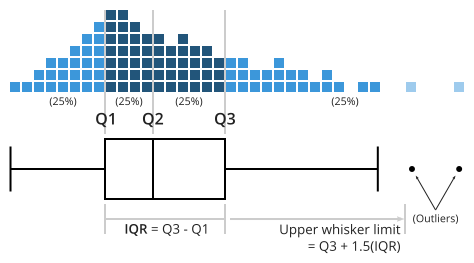
\includegraphics[scale=.35]{clase4-box-plot-construction.png}
\end{center}

\end{frame}


\end{document}

